\chapter{Introduction}
\begin{quote}
At the rate of progress since 1800, every American who lived into the year 2000
would know how to control unlimited power. He would think in complexities
unimaginable to an earlier mind. He would deal with problems altogether beyond
the range of earlier society. To him the nineteenth century would stand on the
same plane with the fourth -- equally childlike -- and he would only wonder how
both of them, knowing so little, and so weak in force, should have done so much.
\attrib{Henry Adams, \textit{The Education of Henry Adams}}
\end{quote}

\begin{quote}
It is change, continuing change, inevitable change, that is the dominant factor
in society today. No sensible decision can be made any longer without taking
into account not only the world as it is, but the world as it will be\ldots
\attrib{Isaac Asimov, \textit{Asimov on Science Fiction}}
\end{quote} 

\newthought{In 1907, Henry Adams published} his autobiography, \textit{The Education of Henry
Adams}. In it, he simultanesouly laments and marvels at the technological change
he has witnessed. When he writes about the impossibility of
understanding it all, his despair is palpable. 

Today, we can only laugh. Too much change? In \textit{1907}? Sure, man taming electricty may have
been a bit of a shock (pun intended), but it was 46 years until it had reached a
quarter of Americans -- more than enough time for the novelty of the thing to
wear off. Childlike, indeed.

Compare that to the inventions since then: It took the telephone 35 years to teach a quarter of Americans, radio
took 31 years, 26 years for television, 16 for the personal computer, 13 for
mobile phones, and a mere 7 for the world wide web.\bigskip

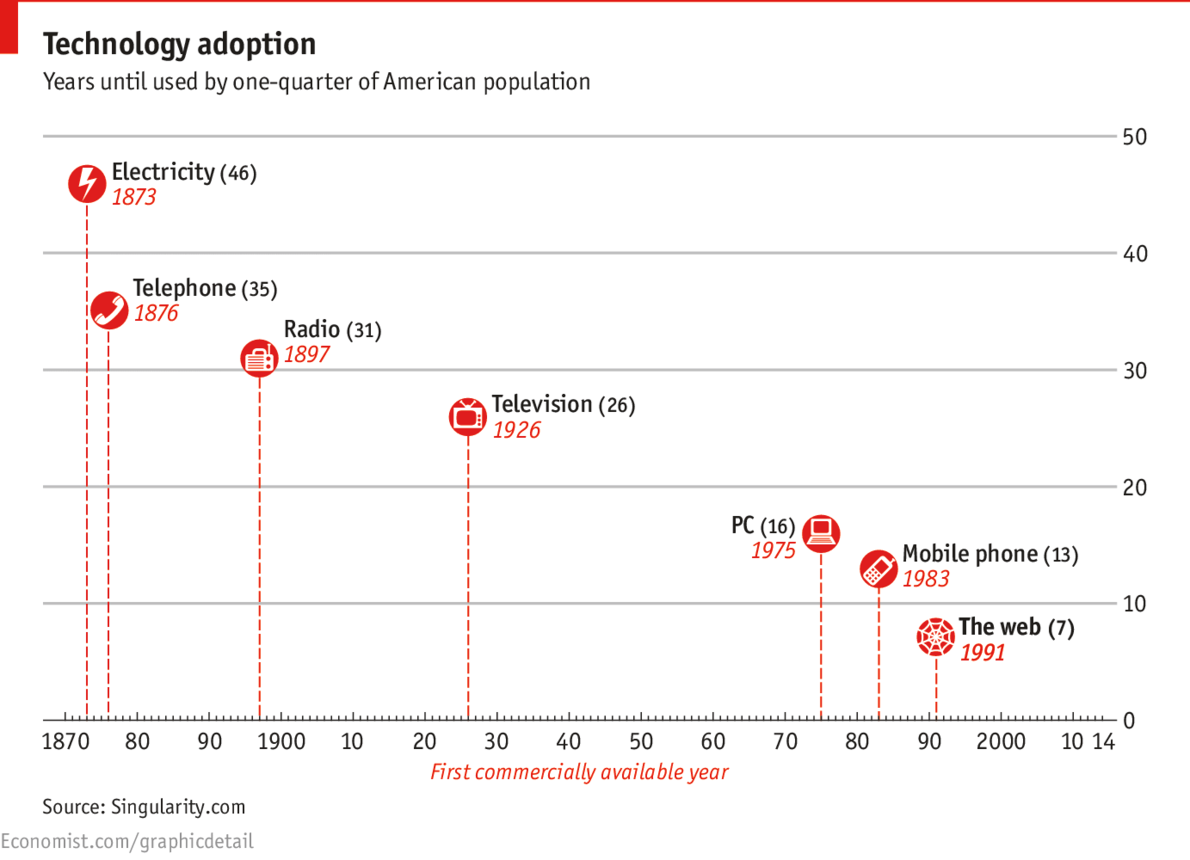
\includegraphics[width=\textwidth]{graphics/accelerating-change}
\bigskip

If we accept, then, that the dissemination of the world wide web and electrity are
roughly comparable, well, some arithmetic suggests that the world is
changing about 6.5x faster today than it was when Henry Adams published his
autobiography. Of course, I'm sure you've felt it -- the constant barrage of the
``next big thing'' that you're tasked with mastering: for web programmers, the
latest and greatest JavaScript framework. For teens, Vine and Snapchat. For
workers generally, your employer's latest iteration of new time tracking
software. 

And this rate of change is accelerating. We're expected to adopt each technology faster than the last.

\newthought{This trend isn't limited to technology.} It's more than
advances like television and radio. In the 13th century, Roger Bacon argued that
it was impossible to master mathematics in less than 30 to 40 years. Today,
roughly equivalent material is routinely taught to high school students.

Sports, too, are no exception. If we transported Olympic swimmers from 1896 to now, they would not even qualify. \cite{ericsson2006influence}

\newthought{Further, consider the sheer amount} of information being produced. About a million books are published each year. That's more books each year than were published
by Western civilization in the sixth, seventh, eighth, ninth, tenth, and
eleventh centuries combined -- a 600 year span. More books were published \textit{just
today} than France did during a 100 year span from the years 600 AD to 700
AD.\cite{buringh2009charting} If that wasn't convincing enough, Google's
executive chairman, Eric Schmidt, estimates that we create more information
every two days than was created from the dawn of civilization until 2003.

There is, then, this expectation that students and workers today will absorb
more and more information in less and less time, and we have no reason to expect
this trend to abate. In fact, it looks as if it will only get worse.

\section{What to expect}

\newthought{Don't panic.} The entire point of this book is to make the world more manageable -- to teach you a few techniques and principles that will supercharge your ability to absorb and retain information. 

In pursuit of this goal, the book is organized into three parts:

\begin{enumerate}
  \item Finding, filtering, and managing external information
  \item Understanding
  \item Retaining knowledge
\end{enumerate}

You'll note that these steps are listed in the order in which they're intended to be enacted.

\newthought{The chapter on} ``Finding, filtering, and managing external
  information'' is on, as you might expect, information gathering. It's a guide
to figuring out what information you need, what it's called, where you can find
it, and how much you should be willing to pay for it.

I want to call information finding ``something of an art,'' but, on reflection,
that's not what I mean. Information finding is a skill. It's a repeatable
process and, with the right instruction and practice, that process can be
refined. I don't know of any skill that a dedicated adult can't
master\footnote{Except maybe perfect pitch.}, and research is something
that one certainly improves over time.

As part of this chapter, I've included several of my most effective techniques
-- the tips and tricks of the trade that I've picked up over the years. This
includes tips for googling, when to dive into the research, where to start,
discovering keywords, and more.

\newthought{The chapter on} ``Understanding'' has also been straightforwardly
named. Once you've found the information you need, you're tasked with
understanding it. This is the process of convering mere information into
knowledge.

Most of the time, understanding something is a straightforward task. However,
the more technical your material leans, or the more unfamiliar with a field you
are, the more obvious and explicit the understanding phase becomes. It feels
like the frustration of not getting something, or of having an ``explicit''
knowledge of a field, but being unable to spontaneously apply that knowledge and
realize just when it's relevant.

In this chapter, I reveal the five most important questions you need to be able to
answer when it comes to really understanding something, and why these questions
work.

\newthought{Finally, the chapter} on ``Retaining knowledge'' covers the basic
principles of human memory, why it's important (in case this is not painfully
obvious), and how these basic principles can be exploited for fun and profit.

It's sometimes claimed that, when you understand something, there is no longer
any need to devote any time to committing it to long-term memory -- that this
crucial step will just spontaneously happen on its own.

This is emphatically not the case. Understanding facillitates remembering, but
it doesn't alleviate the need to manage your own memory. Your memory obeys
certain laws, and these laws cannot be violated.\footnote{Unless you're Kim
  Peek, the real-life inspiration for Dustin Hoffman's role in the movie \textit{Rain Man.} Extreme brain abnoramlities enabled him to instantly commit
  anything to long-term memory. At his death, he'd memorized around 12,000 books.} I'm going to teach this laws and, once aware of
them, you'll better understand why you forget the things that you do forget, and
how you can enhance the effectiveness of your own studying efforts.

\newthought{Enough with} the introduction, then. Let's get started.
